\AtBeginDvi{\special{pdf:mapfile motoya.map}}

\documentclass [10pt] {jsarticle}
%%%% スタイルファイルは各自で用意し自由に使ってください. %%%%
\usepackage[dvipdfmx]{graphicx}
\usepackage{multicol}
\usepackage{url}
\usepackage{comment}
\usepackage{amsmath}
%\usepackage {mystyle}	%% これは架空のスタイルファイル名ですので気をつけて下さい. 
\setlength {\evensidemargin} {-3.5truemm}
\setlength {\oddsidemargin} {-3.5truemm}
\setlength {\footskip} {1.5zw}
\setlength {\headheight} {2zw}
\setlength {\headsep} {0zw}
\setlength{\textheight} {82zw}
\setlength{\textwidth} {50zw}
\setlength{\topmargin} {-20.0truemm}
\renewcommand{\baselinestretch} {0.75}
\renewcommand{\thesection}{\arabic{section}.}
%\renewcommand{\thefigure}{\thesection\arabic{figure}}
\newcommand{\redn} [1] {\textcolor {red}{#1}}
\newcommand{\mrr} [1] {\multirow {3}{*}{#1}}
\makeatletter
\renewcommand {\thetable} {\@arabic\c@section.\@arabic\c@table}
\makeatother
\pagestyle {empty}

\title {\Huge\textgt {タイトル} \vspace {0.5zw} }
\date {}
\author {おなまえ かいてね\\情報電子工学系学科 複雑数理モデル研究室}
\begin {document}
\maketitle
\vspace{-7mm}
\begin{abstract}
これは概要である.この概要でレジュメ全体で何を書いて結論は何かまで書くことが重要となる.このテンプレート作成者は大園 章宏である.特に有益な情報はwikiの個人ページをのぞいても特にない.
\end{abstract}
	%\twocolumn [\maketitle]


\makeatletter
\newenvironment{tablehere}
{\def\@captype{table}}
{}
\newenvironment{figurehere}
{\def\@captype{figure}}
{}

\renewcommand{\thefigure}{%
\thesection\arabic{figure}}
\@addtoreset{figure}{section}



\makeatother

%\begin {document}
\begin{multicols}{2}

\section {はじめに}
論文と同じフォルダ内で作成を行うと画像のパスなどの指定が楽になる.画像のパスの指定はmain.texないしはresume.texといったコンパイルするメインのtexファイルが存在する場所からの相対パスで指定する.\par
句読点は全角コンマ,ピリオドで統一する.vimの変換機能を用いるか入力時に全て変換するかである.揃ってないとカッコ悪い.\par
2段組かつ高さが自動的に揃うため,分量を調整しないと図のキャプションが飛んで行ってしまうことがある.注意する.このテンプレートはカッコ悪い例.

\section{画像について}
画像や表の書き方はfigurehereなとを用いる.使用方法はfigureと変わらないが例を図\ref{pixy}に示す.

\begin{figurehere}
 \begin{center}
  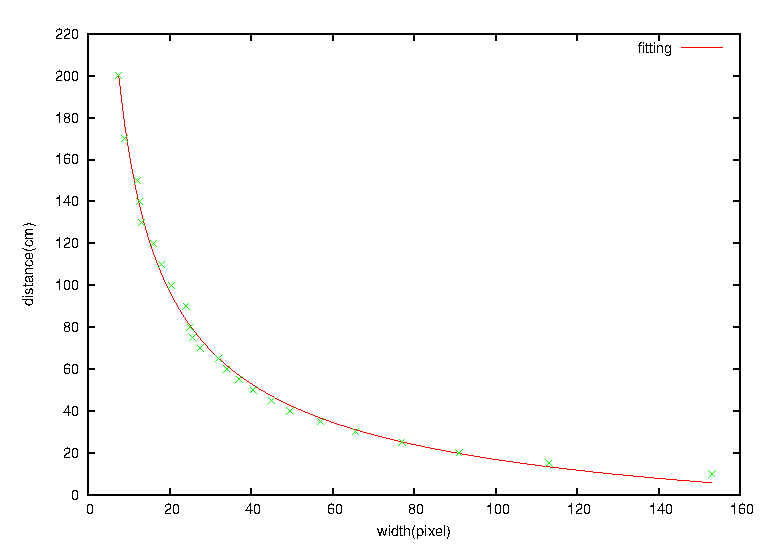
\includegraphics[width=80mm]{appendix/eps/pixy.eps}
  \caption{pixy}
  \label{pixy}
 \end{center}
\end{figurehere}


\section{その他}


\subsection{サブセクション}
サブセクションも使える.



\section{まとめと今後の課題}
最後のセクションの書き方はしっかり考えて欲しい.


\vfill
\begin {thebibliography} {99}
\addcontentsline{toc}{chapter}{\bibname}% タイトル追加
%\bibitem {bib: test}	著者名1, 著者名2, $\dots$, 著者名$n$: 題名, 収録文献名, 収録頁 (掲載年或いは発行年)
\bibitem{a} 浅田稔, 國吉康夫:ロボットインテリジェンス (2006)

\end {thebibliography}


\end{multicols}

\end {document}




